\documentclass[]{article}
\usepackage{lmodern}
\usepackage{amssymb,amsmath}
\usepackage{ifxetex,ifluatex}
\usepackage{fixltx2e} % provides \textsubscript
\ifnum 0\ifxetex 1\fi\ifluatex 1\fi=0 % if pdftex
  \usepackage[T1]{fontenc}
  \usepackage[utf8]{inputenc}
\else % if luatex or xelatex
  \ifxetex
    \usepackage{mathspec}
  \else
    \usepackage{fontspec}
  \fi
  \defaultfontfeatures{Ligatures=TeX,Scale=MatchLowercase}
\fi
% use upquote if available, for straight quotes in verbatim environments
\IfFileExists{upquote.sty}{\usepackage{upquote}}{}
% use microtype if available
\IfFileExists{microtype.sty}{%
\usepackage{microtype}
\UseMicrotypeSet[protrusion]{basicmath} % disable protrusion for tt fonts
}{}
\usepackage[margin=1in]{geometry}
\usepackage{hyperref}
\hypersetup{unicode=true,
            pdftitle={Class 6},
            pdfauthor={Paige Dubelko},
            pdfborder={0 0 0},
            breaklinks=true}
\urlstyle{same}  % don't use monospace font for urls
\usepackage{color}
\usepackage{fancyvrb}
\newcommand{\VerbBar}{|}
\newcommand{\VERB}{\Verb[commandchars=\\\{\}]}
\DefineVerbatimEnvironment{Highlighting}{Verbatim}{commandchars=\\\{\}}
% Add ',fontsize=\small' for more characters per line
\usepackage{framed}
\definecolor{shadecolor}{RGB}{248,248,248}
\newenvironment{Shaded}{\begin{snugshade}}{\end{snugshade}}
\newcommand{\KeywordTok}[1]{\textcolor[rgb]{0.13,0.29,0.53}{\textbf{#1}}}
\newcommand{\DataTypeTok}[1]{\textcolor[rgb]{0.13,0.29,0.53}{#1}}
\newcommand{\DecValTok}[1]{\textcolor[rgb]{0.00,0.00,0.81}{#1}}
\newcommand{\BaseNTok}[1]{\textcolor[rgb]{0.00,0.00,0.81}{#1}}
\newcommand{\FloatTok}[1]{\textcolor[rgb]{0.00,0.00,0.81}{#1}}
\newcommand{\ConstantTok}[1]{\textcolor[rgb]{0.00,0.00,0.00}{#1}}
\newcommand{\CharTok}[1]{\textcolor[rgb]{0.31,0.60,0.02}{#1}}
\newcommand{\SpecialCharTok}[1]{\textcolor[rgb]{0.00,0.00,0.00}{#1}}
\newcommand{\StringTok}[1]{\textcolor[rgb]{0.31,0.60,0.02}{#1}}
\newcommand{\VerbatimStringTok}[1]{\textcolor[rgb]{0.31,0.60,0.02}{#1}}
\newcommand{\SpecialStringTok}[1]{\textcolor[rgb]{0.31,0.60,0.02}{#1}}
\newcommand{\ImportTok}[1]{#1}
\newcommand{\CommentTok}[1]{\textcolor[rgb]{0.56,0.35,0.01}{\textit{#1}}}
\newcommand{\DocumentationTok}[1]{\textcolor[rgb]{0.56,0.35,0.01}{\textbf{\textit{#1}}}}
\newcommand{\AnnotationTok}[1]{\textcolor[rgb]{0.56,0.35,0.01}{\textbf{\textit{#1}}}}
\newcommand{\CommentVarTok}[1]{\textcolor[rgb]{0.56,0.35,0.01}{\textbf{\textit{#1}}}}
\newcommand{\OtherTok}[1]{\textcolor[rgb]{0.56,0.35,0.01}{#1}}
\newcommand{\FunctionTok}[1]{\textcolor[rgb]{0.00,0.00,0.00}{#1}}
\newcommand{\VariableTok}[1]{\textcolor[rgb]{0.00,0.00,0.00}{#1}}
\newcommand{\ControlFlowTok}[1]{\textcolor[rgb]{0.13,0.29,0.53}{\textbf{#1}}}
\newcommand{\OperatorTok}[1]{\textcolor[rgb]{0.81,0.36,0.00}{\textbf{#1}}}
\newcommand{\BuiltInTok}[1]{#1}
\newcommand{\ExtensionTok}[1]{#1}
\newcommand{\PreprocessorTok}[1]{\textcolor[rgb]{0.56,0.35,0.01}{\textit{#1}}}
\newcommand{\AttributeTok}[1]{\textcolor[rgb]{0.77,0.63,0.00}{#1}}
\newcommand{\RegionMarkerTok}[1]{#1}
\newcommand{\InformationTok}[1]{\textcolor[rgb]{0.56,0.35,0.01}{\textbf{\textit{#1}}}}
\newcommand{\WarningTok}[1]{\textcolor[rgb]{0.56,0.35,0.01}{\textbf{\textit{#1}}}}
\newcommand{\AlertTok}[1]{\textcolor[rgb]{0.94,0.16,0.16}{#1}}
\newcommand{\ErrorTok}[1]{\textcolor[rgb]{0.64,0.00,0.00}{\textbf{#1}}}
\newcommand{\NormalTok}[1]{#1}
\usepackage{graphicx,grffile}
\makeatletter
\def\maxwidth{\ifdim\Gin@nat@width>\linewidth\linewidth\else\Gin@nat@width\fi}
\def\maxheight{\ifdim\Gin@nat@height>\textheight\textheight\else\Gin@nat@height\fi}
\makeatother
% Scale images if necessary, so that they will not overflow the page
% margins by default, and it is still possible to overwrite the defaults
% using explicit options in \includegraphics[width, height, ...]{}
\setkeys{Gin}{width=\maxwidth,height=\maxheight,keepaspectratio}
\IfFileExists{parskip.sty}{%
\usepackage{parskip}
}{% else
\setlength{\parindent}{0pt}
\setlength{\parskip}{6pt plus 2pt minus 1pt}
}
\setlength{\emergencystretch}{3em}  % prevent overfull lines
\providecommand{\tightlist}{%
  \setlength{\itemsep}{0pt}\setlength{\parskip}{0pt}}
\setcounter{secnumdepth}{0}
% Redefines (sub)paragraphs to behave more like sections
\ifx\paragraph\undefined\else
\let\oldparagraph\paragraph
\renewcommand{\paragraph}[1]{\oldparagraph{#1}\mbox{}}
\fi
\ifx\subparagraph\undefined\else
\let\oldsubparagraph\subparagraph
\renewcommand{\subparagraph}[1]{\oldsubparagraph{#1}\mbox{}}
\fi

%%% Use protect on footnotes to avoid problems with footnotes in titles
\let\rmarkdownfootnote\footnote%
\def\footnote{\protect\rmarkdownfootnote}

%%% Change title format to be more compact
\usepackage{titling}

% Create subtitle command for use in maketitle
\newcommand{\subtitle}[1]{
  \posttitle{
    \begin{center}\large#1\end{center}
    }
}

\setlength{\droptitle}{-2em}

  \title{Class 6}
    \pretitle{\vspace{\droptitle}\centering\huge}
  \posttitle{\par}
    \author{Paige Dubelko}
    \preauthor{\centering\large\emph}
  \postauthor{\par}
      \predate{\centering\large\emph}
  \postdate{\par}
    \date{January 24, 2019}


\begin{document}
\maketitle

\subsubsection{Section 1: Reading files}\label{section-1-reading-files}

We are using the \textbf{read.table()} funtion and friends to read some
example flat files.

\begin{Shaded}
\begin{Highlighting}[]
\KeywordTok{read.csv}\NormalTok{(}\StringTok{"test1.txt"}\NormalTok{)}
\end{Highlighting}
\end{Shaded}

\begin{verbatim}
##   Col1 Col2 Col3
## 1    1    2    3
## 2    4    5    6
## 3    7    8    9
## 4    a    b    c
\end{verbatim}

For the test1 file, we are able to use read.table(), but because we
notice it is separated by ``,'' and appears to have a header, the
\textbf{read.csv} is a simpler option.

We will now look at our \textbf{second} text file\ldots{} We see that
this file is separated by `\$' and has a header.

\begin{Shaded}
\begin{Highlighting}[]
\KeywordTok{read.table}\NormalTok{(}\StringTok{"test2.txt"}\NormalTok{, }\DataTypeTok{header =} \OtherTok{TRUE}\NormalTok{, }\DataTypeTok{sep =} \StringTok{"$"}\NormalTok{)}
\end{Highlighting}
\end{Shaded}

\begin{verbatim}
##   Col1 Col2 Col3
## 1    1    2    3
## 2    4    5    6
## 3    7    8    9
## 4    a    b    c
\end{verbatim}

Because we do not have a friend function that separates by ``\$'' it is
easy to edit table to specify it for this file.

Now onto the \textbf{third} file. We notice that the data is separated
by what looks like spaces and does not have a header. So we just use the
\textbf{read.table()} function.

\begin{Shaded}
\begin{Highlighting}[]
\KeywordTok{read.table}\NormalTok{(}\StringTok{"test3.txt"}\NormalTok{)}
\end{Highlighting}
\end{Shaded}

\begin{verbatim}
##   V1 V2 V3
## 1  1  6  a
## 2  2  7  b
## 3  3  8  c
## 4  4  9  d
## 5  5 10  e
\end{verbatim}

\subsubsection{Section 2: R Functions}\label{section-2-r-functions}

Lets write a simple function, add()\ldots{}

\begin{Shaded}
\begin{Highlighting}[]
\NormalTok{add <-}\StringTok{ }\ControlFlowTok{function}\NormalTok{(x,}\DataTypeTok{y=}\DecValTok{1}\NormalTok{)\{}
  \CommentTok{#Sum the input x and y}
\NormalTok{  x }\OperatorTok{+}\StringTok{ }\NormalTok{y}
\NormalTok{\}}
\end{Highlighting}
\end{Shaded}

Now lets try add()!

\begin{Shaded}
\begin{Highlighting}[]
\NormalTok{x <-}\StringTok{ }\DecValTok{7}
\NormalTok{y <-}\StringTok{ }\DecValTok{3}
\KeywordTok{add}\NormalTok{(}\DecValTok{7}\NormalTok{,}\DecValTok{3}\NormalTok{)}
\end{Highlighting}
\end{Shaded}

\begin{verbatim}
## [1] 10
\end{verbatim}

We are also able to use our add function with vectors :) Remember: the y
variable is optional.

\begin{Shaded}
\begin{Highlighting}[]
\KeywordTok{add}\NormalTok{(}\KeywordTok{c}\NormalTok{(}\DecValTok{1}\NormalTok{,}\DecValTok{2}\NormalTok{,}\DecValTok{3}\NormalTok{))}
\end{Highlighting}
\end{Shaded}

\begin{verbatim}
## [1] 2 3 4
\end{verbatim}

If you find yourself doing the same thing three or more times, it might
be time to think about writing a function.

\textbf{2nd Function: Rescale}

\begin{Shaded}
\begin{Highlighting}[]
\NormalTok{rescale <-}\StringTok{ }\ControlFlowTok{function}\NormalTok{(x)\{}
\NormalTok{  rng <-}\StringTok{ }\KeywordTok{range}\NormalTok{(x)}
\NormalTok{  (x }\OperatorTok{-}\StringTok{ }\NormalTok{rng[}\DecValTok{1}\NormalTok{]) }\OperatorTok{/}\StringTok{ }\NormalTok{(rng[}\DecValTok{2}\NormalTok{] }\OperatorTok{-}\StringTok{ }\NormalTok{rng[}\DecValTok{1}\NormalTok{])}
\NormalTok{\}}
\end{Highlighting}
\end{Shaded}

Lets test on a small example, where we know what the answer should be

\begin{Shaded}
\begin{Highlighting}[]
\KeywordTok{rescale}\NormalTok{(}\DecValTok{1}\OperatorTok{:}\DecValTok{10}\NormalTok{)}
\end{Highlighting}
\end{Shaded}

\begin{verbatim}
##  [1] 0.0000000 0.1111111 0.2222222 0.3333333 0.4444444 0.5555556 0.6666667
##  [8] 0.7777778 0.8888889 1.0000000
\end{verbatim}

With how it is currently written, our rescale function will not take NA
values, so we must change it.

\begin{Shaded}
\begin{Highlighting}[]
\NormalTok{rescale2 <-}\StringTok{ }\ControlFlowTok{function}\NormalTok{(x)\{}
\NormalTok{  rng <-}\StringTok{ }\KeywordTok{range}\NormalTok{(x, }\DataTypeTok{na.rm =} \OtherTok{TRUE}\NormalTok{)}
\NormalTok{  (x }\OperatorTok{-}\StringTok{ }\NormalTok{rng[}\DecValTok{1}\NormalTok{]) }\OperatorTok{/}\StringTok{ }\NormalTok{(rng[}\DecValTok{2}\NormalTok{] }\OperatorTok{-}\StringTok{ }\NormalTok{rng[}\DecValTok{1}\NormalTok{])}
\NormalTok{\}}
\end{Highlighting}
\end{Shaded}

This will now work for vectors containing NA values because we set
\textbf{na.rm} equal to TRUE

\begin{Shaded}
\begin{Highlighting}[]
\NormalTok{x <-}\StringTok{ }\KeywordTok{c}\NormalTok{(}\DecValTok{1}\NormalTok{,}\DecValTok{2}\NormalTok{,}\OtherTok{NA}\NormalTok{,}\DecValTok{3}\NormalTok{,}\DecValTok{10}\NormalTok{)}
\KeywordTok{rescale2}\NormalTok{(x)}
\end{Highlighting}
\end{Shaded}

\begin{verbatim}
## [1] 0.0000000 0.1111111        NA 0.2222222 1.0000000
\end{verbatim}

Lets edit this function one more time.

\begin{Shaded}
\begin{Highlighting}[]
\NormalTok{rescale3 <-}\StringTok{ }\ControlFlowTok{function}\NormalTok{(x, }\DataTypeTok{na.rm =} \OtherTok{TRUE}\NormalTok{, }\DataTypeTok{plot =} \OtherTok{FALSE}\NormalTok{)\{}
\NormalTok{  rng <-}\StringTok{ }\KeywordTok{range}\NormalTok{(x, }\DataTypeTok{na.rm =}\NormalTok{ na.rm)}
  \KeywordTok{print}\NormalTok{(}\StringTok{"Hello"}\NormalTok{)}
  
\NormalTok{  answer <-}\StringTok{ }\NormalTok{(x }\OperatorTok{-}\StringTok{ }\NormalTok{rng[}\DecValTok{1}\NormalTok{]) }\OperatorTok{/}\StringTok{ }\NormalTok{(rng[}\DecValTok{2}\NormalTok{] }\OperatorTok{-}\StringTok{ }\NormalTok{rng[}\DecValTok{1}\NormalTok{])}
  
  \KeywordTok{print}\NormalTok{(}\StringTok{"is it me you are looking for?"}\NormalTok{)}
  
  \ControlFlowTok{if}\NormalTok{(plot)\{}
    \KeywordTok{plot}\NormalTok{(answer, }\DataTypeTok{typ =} \StringTok{"b"}\NormalTok{, }\DataTypeTok{lwd =} \DecValTok{4}\NormalTok{)}
\NormalTok{  \}}
  \KeywordTok{print}\NormalTok{(}\StringTok{"I can see it in ..."}\NormalTok{)}
  \KeywordTok{return}\NormalTok{(answer)}
\NormalTok{\}}
\end{Highlighting}
\end{Shaded}

Lets try it!

\begin{Shaded}
\begin{Highlighting}[]
\KeywordTok{rescale3}\NormalTok{(}\KeywordTok{c}\NormalTok{(}\DecValTok{1}\OperatorTok{:}\DecValTok{6}\NormalTok{), }\DataTypeTok{plot =} \OtherTok{TRUE}\NormalTok{)}
\end{Highlighting}
\end{Shaded}

\begin{verbatim}
## [1] "Hello"
## [1] "is it me you are looking for?"
\end{verbatim}

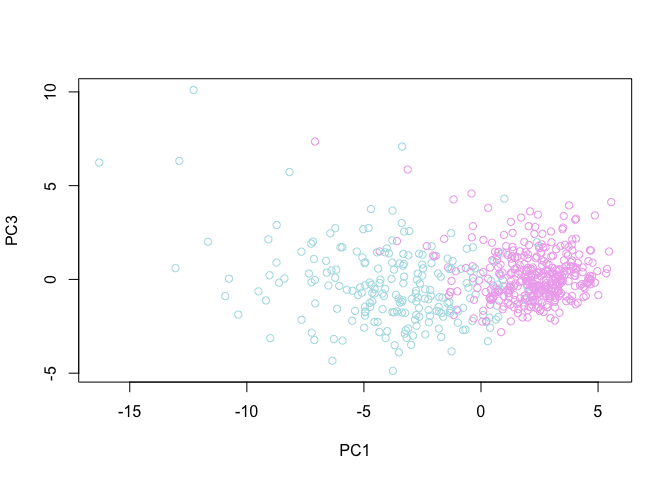
\includegraphics{class06_files/figure-latex/unnamed-chunk-12-1.pdf}

\begin{verbatim}
## [1] "I can see it in ..."
\end{verbatim}

\begin{verbatim}
## [1] 0.0 0.2 0.4 0.6 0.8 1.0
\end{verbatim}


\end{document}
